\documentclass[11pt]{article}
\usepackage{amsfonts}
\usepackage[yyyymmdd,hhmmss]{datetime}
\usepackage{amsmath}
\usepackage{cancel}
\usepackage{mathtools}
\usepackage{graphicx}
\usepackage{multirow}
\usepackage{caption}
\usepackage{subcaption}

\setlength{\pdfpagewidth}{8.5in}
\setlength{\pdfpageheight}{11in}
\textwidth 6.5in
\textheight 9in
\headheight 0.0in
\topmargin -.5in
\oddsidemargin 0.0in
\evensidemargin 0.0in

\title{\bf CS 186 - Homework 3}
\date{\today}
\author{Matthew Warshauer \& Ye Zhao}
\begin{document}
\maketitle
\section{Designing a bidding agent}
See implmentation in code distribution.
\section{Analysis of the GSP agents}
\subsection{Average Utility}
We run the simulation for either 5 truthful agents or 5 balanced budget (mewzybb) agents with seed 5 and 200 iterations. The total utility for the two scenarios are shown below
\begin{itemize}
\item Truthful Agent: $u_{tot}=\$1659.37$
\item Balanced Agent (mewzybb): $u_{tot}=\$3342.55$
\end{itemize}
There is a improvement of \$1683.18 or approximately 67.3\%.
\\
\\
We see that the balanced bidding agents result in a better total utility of the bidding. This is because truthfulness is not an equilbrium in the generalized second price auction, while balanced bidding is an equilibrium. Switching from all truthful to all balanced bidding is a pareto improvement.
\subsection{Truthful vs Balanced Bidding}
We again run the simulation with seed 5, permutation 10 and 200 iterations, the results are shown below:
\begin{itemize}
	\item 4 truthful agents \& 1 balanced bidding agent
		\begin{center}
		\begin{tabular}{| c | c | c | c | c | }
			\hline
			Truthful 1 & Truthful 2 & Truthful 3 & Truthful 4 & BB 1\\ \hline
			\$371.94 & \$356.79 & \$356.18 & \$348.80 & \$577.03 \\ \hline
		\end{tabular}
		\end{center}
	\item 1 truthful agent \& 4 balanced bidding agents
		\begin{center}
		\begin{tabular}{| c | c | c | c | c | }
			\hline
			Truthful 1 & BB 1 & BB 2 & BB 3 & BB 4 \\ \hline
			\$647.75 & \$646.91 & \$641.80 & \$631.33 & \$651.80 \\ \hline
		\end{tabular}
		\end{center}
\end{itemize}
The results show that for the first case of 4 truthful agents and 1 balanced bidding agent, the balanced bidding agent performed better than the rest with an average utility of \$577.03 and for the second case of 1 truthful agents and 4 balanced bidding agents, every single agents average utilities were of comparable level.
\\
\\
This suggests that when everyone is playing truthful bidding, there is an incentive for an agent to deviate away from playing truthful and play balanced bidding instead, whereas when everyone is playing balanced bidding, playing truthful doesn't changed the expected utility of the game.
\section{Auction Design and Reserve Prices}
\subsection{Revenue under GSP with various reserve price}
With no reserve price and all agents using balanced bidding under GSP the auctioneer's revenue is $\$4713.48$. As the reserve price increases, the revenue of the auctioneer increases, but only for a limited time. At a certain point (in this case around $80$ cents) the revenue begins to decline again as the reserve price forces too many bidders out of the auction. This behavior can be observed in the following graph.
\subsection{Implement VCG}
The following is our implementation of the payment rule, which in conjunction with the distribution code fully implements the VCG auction.
\begin{verbatim}
        def total_payment(k):
            """
            Total payment for a bidder in slot k.
            """
            c = slot_clicks
            n = len(allocation)

            # TODO: Compute the payment and r eturn it.
            if k == n - 1:
                if len(valid_bids) == n:
                    return c[k] * reserve
                (_, next_highest_bid) = valid_bids[n]
                return c[k] * max(reserve, next_highest_bid)
            else:
                return (c[k] - c[k + 1]) * just_bids[k + 1] + total_payment(k + 1)
\end{verbatim}
\subsection{Revenue under VCG}
With no reserve price and all agents using truthful bidding under VCG the auctioneer's revenue is $\$4530.65$. As the reserve price increases, the revenue of the auctioneer increases, but only for a limited time. At a certain point (in this case again around $80$ cents) the revenue begins to decline again as the reserve price forces too many bidders out of the auction. This behavior can be observed in the above graph. This is exceedingly similar to the results in part a, which makes sense given that balanced bidding under GSP produces the same equilibrium outcome as truthful bidding under VCG.
\begin{figure}[h]
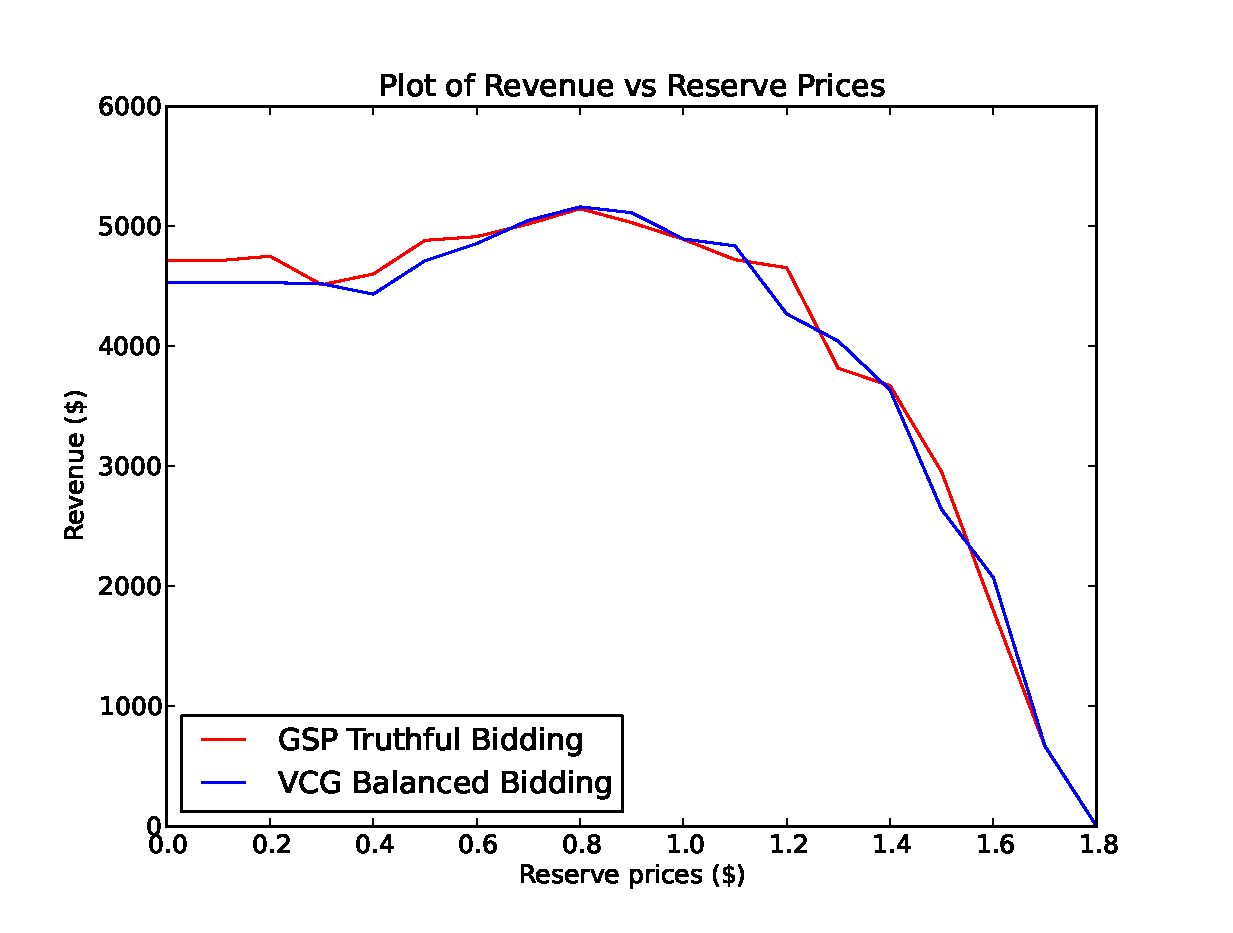
\includegraphics[width=\textwidth]{revenue_plot.eps}
\caption{Plot of Revenue vs Reserve Prices}
\end{figure}
\subsection{Switching midstream}
With a reserve price of $0$, a switch from GSP to VCG at round $24$ and all agents using balanced bidding causes a revenue of $\$4275.20$. This is less than the $\$4713.48$ they would have gotten from sticking with GSP (see part a).
\subsection{Bigger picture}
These exercises have demonstrated to us the theory that different strategies under different auction structures can behave identically in equilibrium outcome. We saw how different auction structures lead to varying complex rules of bidding, allocation, and payment. This was also a valuable example of the Revenue Equivalence Theorem in practice. Finally, we saw one possible reason why Google and other sites that sell ads with GSP might be hesistant to switch to VCG. If they were to switch, bidders might not immediately switch to the truthful strategy and they would lose money during the period of adjustment.   


\section{Budget constraints}
\end{document}
